\documentclass[a4paper, 11pt]{report}

%%%% Packages %%%%
\usepackage[utf8]{inputenc}
\usepackage[francais]{babel}
\usepackage{framed}
\usepackage{amssymb}
\usepackage{verbatim}
\usepackage{listings}
\usepackage[hidelinks]{hyperref}

\usepackage[usenames,dvipsnames,table,xcdraw]{xcolor}
\usepackage[pdftex]{graphicx}
\usepackage{sectsty}

%% Couleurs
 \definecolor{orange}{HTML}{E74C3C}
 \definecolor{dark-blue}{HTML}{1A2530}
 \definecolor{blue}{HTML}{34495E}
 \definecolor{dkgreen}{rgb}{0,0.6,0}
 \definecolor{gray}{rgb}{0.5,0.5,0.5}
 \definecolor{mauve}{rgb}{0.58,0,0.82}
 
  \definecolor{part_color}{HTML}{E74C3C}
   \definecolor{section_color}{HTML}{2C3E50}
    \definecolor{subsection_color}{HTML}{34495E}
 
 
 \colorlet{shadecolor}{gray!7}

%% Parametres
\setcounter{tocdepth}{1}
\setlength{\parindent}{0pt}
\partfont{\color{part_color}}
\sectionfont{\color{section_color}}
\subsectionfont{\color{subsection_color}}
\makeatletter
\@addtoreset{section}{part}
\makeatother  


%% Commandes
\renewcommand{\thesection}{\Roman{section}}
\renewcommand{\thesubsection}{\arabic{subsection}} % Les sections n'affichent pas le numero du chapitre

\newcommand{\HRule}{\rule{\linewidth}{0.5mm}}
%% Environements
\renewenvironment{shaded}
	{
  	\def\FrameCommand{\fboxsep=\FrameSep \colorbox{shadecolor}
  	}
  	\MakeFramed{\advance\hsize-\width \FrameRestore\FrameRestore}}
 {\endMakeFramed}
 
 \lstset{frame=tb,
  language=Java,
  aboveskip=3mm,
  belowskip=3mm,
  showstringspaces=false,
  columns=flexible,
  basicstyle={\small\ttfamily},
  numbers=none,
  numberstyle=\tiny\color{gray},
  keywordstyle=\color{blue},
  commentstyle=\color{dkgreen},
  stringstyle=\color{mauve},
  breaklines=true,
  breakatwhitespace=true,
  tabsize=3
}

    
\newenvironment{vulgarisation}
    {
    \textit{\textcolor{dark-blue}{$\blacksquare$  Vulgarisation : \\}}

    }
    {
    ~\\\textcolor{dark-blue}{$\blacksquare$}\\
    }
    
\newenvironment{formalisation}
    {
    \textit{\textcolor{blue}{$\blacksquare$  Formalisation : \\}}
    }
    {
    ~\\\textcolor{blue}{$\blacksquare$}\\
    }
    
\newenvironment{codage}
    {
    \textit{\textcolor{gray}{$\blacksquare$  Règle JAPE : \\}}
    }
    {
    ~\\\textcolor{gray}{$\blacksquare$}\\
    }
    
\newenvironment{exemple}
    {
    \textit{\textcolor{orange}{
    Exemple : \\}}
    }
    {\\
    }

\begin{document}

%% Couverture
\author{Charles Follet \and Roland Bary}

\begin{titlepage}
\begin{center}

% Upper part of the page. The '~' is needed because \\
% only works if a paragraph has started.

\includegraphics[width=0.25\textwidth]{./logo.png}~\\[1cm]

\textsc{\Large Projet Tutoré}\\[0.5cm]
\textsc{\Large M1 Technologies de l'Internet}\\[0.5cm]

% Title
\HRule \\[0.4cm]
{ \LARGE \bfseries Conception et développement d’une application d’annotation thématique dans
l'environnement Gate \\[0.4cm] }

\HRule \\[1.5cm]

% Author and supervisor
\noindent
\begin{minipage}[t]{0.4\textwidth}
\begin{flushleft} \large
\emph{Auteurs:}\\
Roland \textsc{Bary}\\
Charles \textsc{Follet}
\end{flushleft}
\end{minipage}%
\begin{minipage}[t]{0.4\textwidth}
\begin{flushright} \large
\emph{Tuteurs:} \\
Marie-Noëlle \textsc{Bessagnet}\\
Annig \textsc{Lacayrelle}\\
Albert \textsc{Royer}\\
Christian \textsc{Sallaberry}
\end{flushright}
\end{minipage}

\vfill

% Bottom of the page
{\large \date{}}

\end{center}
\end{titlepage}
\section*{Remerciements}
Nous tenons à remercier nos tuteurs pour leur pédagogie et leur encadrement. Monsieur Royer pour sa précision et sa connaissance pointue du domaine. Madame Lacayrelle pour son soutien et sa clarté. Monsieur Sallaberry pour nous avoir remis sur de bonnes pistes quand nous nous égarions. Et enfin, madame Bessagnet pour avoir assuré la coordination et le suivi de ce projet.
\tableofcontents

\part{Introduction}
L'évolution des volumes d'informations sur internet provoque une évolution du web vers une approche dans laquelle chaque donnée acquiert un sens afin de rendre possible une interprétation du contenu par des machines. Cette évolution constitue le web sémantique.\\
Sa principale motivation  est la recherche d’information sémantique.\\

Dans ce cadre, nous sommes intervenus pour répondre à l'appel d'offre de la maîtrise d'ouvrage. \\
L'objectif correspond à la première étape dans un processus de recherche d'informations sémantiques et d'indexation : l'annotation sémantique d'un document texte spécifique.\\

En découle les problématiques suivantes :
\begin{itemize}
\item Existe-t-il des outils qui se prêtent aisément à l'annotation sémantique ?
\item Quelle approche de conception nous permet de réaliser cette étape d'annotation sur un document texte non-structuré ?
\end{itemize}
	~\\
	
La résolution de ces différentes problématiques nous a amenés à organiser notre réflexion :\\
Premièrement, nous définirons clairement les demandes et leurs contextes à travers le cahier des charges. Deuxièmement, nous présenterons l'état des connaissances actuelles sur le sujet. Troisièmement, nous détaillerons notre principe de résolution du projet. Nous finirons le bilan et le retour d’expérience de ce projet.
\part{Cahier des charges}
	\section{Contexte}

A partir des travaux de Georges DEPEYROT sur les monnaies carolingiennes, nous avons travaillé pour une équipe parisienne de numismates sur l'annotation du Numéraire Carolingien\footnote{\url{http://www.cgb.fr/le-numeraire-carolingien-moneta-77-3e-edition-depeyrot-georges,Ln71,a.html}}.\\
Sur celui-ci, l'équipe a besoin d'effectuer des recherches :

\begin{description}
\item [Temporelles] : Quelles étaient les pièces en circulation de l'an 859 à l'an 865?
\item [Spatiales] : Dans quels ateliers, les pièces de type Obole de Charlemagne ont été produites ? 
\item [Thématiques] : Combien d'exemplaires de la monnaie d'or de Charles le Chauve ont été étudiés ?
\end{description}

Répondre à cette demande implique de définir puis d'explorer les dimensions temporelles, spatiales et thématiques de l'ouvrage.\\
Pour cela, il est nécessaire de connaître le domaine et l'ouvrage afin de savoir quelle information correspond à quelle dimension.\\
Une fois cet apprentissage fait, nous pouvons construire des règles dans une chaine de traitement permettant d'annoter chaque information en fonction de sa dimension. \\

Les monnaies carolingiennes sont le domaine central pour la réalisation du projet. Les ressources nécessaires à l'annotation (ici sous forme de gazetiers) ont été construites à partir des données de l'ouvrage.\\

Forte de son expérience dans le domaine, la maîtrise d'ouvrage nous a demandé d'utiliser la boîte à outils logicielle GATE qui sera utile pour le traitement du langage naturel.\\~\\

En résumé, les caractéristiques du projet sont : 
\begin{itemize}
\item l'apprentissage et la compréhension du domaine considéré,
\item l'étude des principes d'annotation de documents,
\item le développement d'une chaîne d'annotation dans GATE,
\item la mise en place d'une visualisation des résultats.
\end{itemize}

\newpage
	\section{Description}
	
	La chaine de traitement prend un document textuel en entrée, produit un document XML en sortie et le met en forme pour une meilleure lisibilité.\\
	\begin{exemple}
\noindent Illustrons par un scénario les objectifs de la chaîne de traitement.
Elle prend par exemple en entrée le texte suivant

\begin{figure}[h!]
\centering
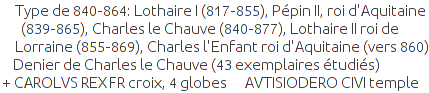
\includegraphics[scale=.5]{img/exemple_text.png}
\end{figure}

et l'annote
\end{exemple}
\begin{figure}[h!]
\centering
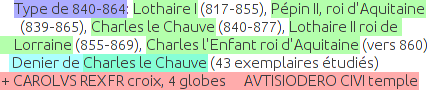
\includegraphics[scale=.5]{img/exemple_text_ann.png} 
\end{figure}\\
Chaque information pertinente est annotée. En bleu la période d'émission de la monnaie (Temporel), en vert les souverains qui l'ont faite produire (Thématique), en cyan la nature de la monnaie (Thématique) et en rouge la légende (Thématique).\\
Afin de développer cette chaîne,nous avons dû planifier notre travail et nos réunions avec la maîtrise d'ouvrage. Cette planification sera présentée dans la partie suivante.

	\section{Diagramme de Gantt prévisionnel}
	
\part{Cadre d'analyse}
	\section*{Introduction}
	
	\section{Définition de concepts}
	
		\subsection{Gazetier}
		
		\subsection{Entité nommée}
		
		\subsection{Expression régulière}
		
	\section{Outil}
	
		\subsection{L'environnement Gate}
		



\part{Développement}
	\section*{Introduction}
	Avant de démarrer le développement de la chaîne de traitement, nous devons nous familiariser avec notre environnement de travail. Celui-ci comprend l'outil GATE et le Numéraire carolingien. Ensuite, nous allons pouvoir définir nos annotations, leur domaine et choisir de quelle façon nous allons les capturer.
	\section{Prise en main de l'environnement}
	\subsection{GATE}

	\subsection{Numéraire Carolingien}
	Au lancement du projet, la seule ressource a disposition été le Numéraire Carolingien au format papier. Il fallait le numériser et l'OCRiser.\\
    Nous avons numérisé une cinquantaine de pages à la main pour les OCRiser automatiquement par la suite à l'aide de l'outil \texttt{tesseract}.\\

    L'OCRisation s'est déroulée de la façon suivante : 
    \begin{figure}[h]
    \centering
    
\includegraphics[scale=.3]{img/OCRisation.png}
    \end{figure}\\
    La scanner que nous avons utilisé permettait d'obtenir une image pour chacune des pages au format PDF. Ensuite, étant donné que  \texttt{tesseract} est plus performant et précis avec des fichiers TIFF, il a fallu convertir les fichiers PDF en TIFF. Cependant, quelques erreurs d'OCRisation sont apparues. Pour finir,  \texttt{tesseract} nous donnait des fichiers TXT.\\
    Les étapes de conversion du schéma précédent ont été réalisées à l'aide de script en langage SHELL:
    \begin{enumerate}
        \item \begin{enumerate}
    	      \item	
           \begin{verbatim}
for file in *.pdf
do
  convert -density 300 ../pdf/$file -depth 8 `basename $file .pdf`.tiff
done
           \end{verbatim}
          \item les pages impaires ont été numérisée à l'envers, il fallait les mettre dans le bon sens.
          \begin{verbatim}
for file in *.tiff
do
    if [ $((`basename $file .tiff` % 2 )) = 1 ]; then
        convert $file -rotate 180 $file;
    fi
done
          \end{verbatim}
       \end{enumerate}
    \item 
    \begin{verbatim}
for file in img/*.tiff
do
  tesseract $file txt/`basename $file .tiff` -l fra
done 
    \end{verbatim}
    \end{enumerate}
    
	\section{Définition des dimensions d'annotation et leur contenu}
    Dans l'introduction, nous avons vu qu'il y a trois dimensions d'annotation.\\


    
    \subsection{Dimension spatiale}
    \subsubsection{Définition}
     La dimension spatiale contient toutes les informations de lieux. Peu spécifique au domaine considéré.
    \subsubsection{Contenu}
       Le contenu de cette dimension est minime. Hormis les ateliers, les lieux présents dans le document n'intéressent que très peu la maîtrise d'ouvrage.
	\subsection{Dimension temporelle}
	    \subsubsection{Définition}
    La dimension temporelle contient toutes les informations de temps et de durées. Peu spécifique au domaine considéré.\\
    \subsubsection{Contenu}
    \begin{description}
    \item[les périodes d'émission]... TODO
    \end{description}
    

	\subsection{Dimension thématique}
	    \subsubsection{Définition}
    La dimension thématique contient toutes les informations du domaine considéré. 
    \subsubsection{Contenu}	
    
    
    
	\section{Première recherche d'entités nommées avec les gazetiers}
	\subsubsection{Ateliers}
\begin{vulgarisation}
	L'ouvrage est décomposé en ateliers qui donnent leur nom à chaque début de "partie" ou "chapitre". Ce nom correspond à un endroit de France ou pays limitrophes dans lequel est produite la monnaie. Ce lieu peut être une ville, un lieu-dit dont le nom peut ne plus exister. Il fût donc difficile de trouver un pattern via les expressions régulières. Nous avons alors dû construire ce gazetier à partir de la liste en début d'ouvrage qui recense tous les ateliers.
\end{vulgarisation}
\begin{formalisation}
\begin{verbatim}
Aix-la-Chapelle (Allemagne)
Agen (Lot-et-Garonne)
Aix-la-Chapelle
Alsheim (Allemagne)
Altenheim (Bas-Rhin)
Amiens (Somme)
\end{verbatim}
\end{formalisation}

\subsubsection{Souverains}
\begin{vulgarisation}
	Le nom des souverains ont des formats aussi divers que variés.Ils comportent des majuscules, des chiffres romains... Il serait difficile d'utiliser une expression régulière pour espérer annoter cette information. Il est plus judicieux d'utiliser un gazetier. Il sera construit à partir du début du numéraire. 
\end{vulgarisation}
\begin{formalisation}
\begin{verbatim}
Pépin le Bref:valeur=Pépin le Bref:periode=752-768
Adalbert Lothaire:valeur=Adalbert Lothaire:periode=954-986
Amoul roi de Germanie:valeur=Amoul roi de Germanie:periode=887-899
Bérenger I:valeur=Bérenger I:periode=888-924
Bérenger II:valeur=Bérenger II:periode=950-961
\end{verbatim}
\end{formalisation}

	\section{Deuxième recherche d'entités nommées avec les règles JAPE}
	\subsubsection{Périodes}
\begin{vulgarisation}
	\textit{Période} : intervalle de deux dates séparées par un tiret.\\
	\begin{exemple}
		\textit{757/8-786}
	\end{exemple}
	
	Une période est un intervalle entre deux dates. Dans notre travail, les dates sont constituées de trois et seulement trois chiffres. En cas d'ambiguïté,Chacune d'elle peut être suivie d'un \og/\fg{} et d'un chiffre traduisant l'indétermination de la date.\\
	\begin{exemple}
		\textit{757/8}
	\end{exemple}
	
\end{vulgarisation}
\begin{formalisation}
	\textit{Date}
	\begin{verbatim}
([0-9]{3}\/?[0-9]?)
	\end{verbatim}
	\textit{Période}
	\begin{verbatim}
([0-9]{3}(\/[0-9])?)-([0-9]{3}(\/[0-9])?)
	\end{verbatim}
	\begin{exemple}
		"\emph{Type de 771-793/4: Charlemagne (768-814),...}" \\
		Group \#1 : 771 \\
		Group \#2 : 793/4\\\\\noindent
		Group \#1 : 768 \\
		Group \#2 : 814
	\end{exemple}
\end{formalisation}
	\begin{codage}
	\begin{lstlisting}
		// Regle JAPE
	Macro: TROIS_NOMBRES
({Token.kind==number,Token.length == 3})

Macro: UN_NOMBRE
({Token.kind==number,Token.length == 1})

Macro:SLASH
({Token.string=="/"})

Macro:DATE_PRECISE
(TROIS_NOMBRES)

Macro:DATE_IMPRECISE
(TROIS_NOMBRES SLASH UN_NOMBRE)

Macro:DATE
(DATE_PRECISE | DATE_IMPRECISE)

Rule: PeriodeRule
(
	(DATE):d1({Token.string =="-"})(DATE):d2
    ):Periode -->
:Periode{/*Code java pour extraire les extremites de l'intervalle*/}
	\end{lstlisting}
	\end{codage}
	
\newpage
\subsubsection{Périodes d'émission}
\begin{vulgarisation}
	Une période d'émission a la forme suivante :  \og Type de \{Période\} : \fg{} (Période étant l'annotation définie précédemment).\\
	Il faut sécuriser la capture de la période d'émission en ajoutant la contrainte précédée de "Type de" afin de ne pas récupérer toutes les périodes du documents.
\end{vulgarisation}
\begin{formalisation}
	\begin{verbatim}
Type de : ([0-9]{3}(\/[0-9])?)-([0-9]{3}(\/[0-9])?)
	\end{verbatim}
	\begin{exemple}
		"\emph{Type de 771-793/4: Charlemagne (768-814)...}" \\
		Group \#1 : 771 \\
		Group \#2 : 793/4
	\end{exemple}

\end{formalisation}
			\begin{codage}
	\begin{lstlisting}
	// Regle JAPE
	Macro: CHAINE_DEBUT
(
    ({Token.string =="Type"})({SpaceToken})
    ({Token.string =="de"})({SpaceToken})
)

Rule: PeriodeEmissionRule
(
    CHAINE_DEBUT ({Periode}):p
):PeriodeEmission
-->
:PeriodeEmission.PeriodeEmission = { Kind = "PeriodeEmission" ,D1 = :p.Periode.D1, D2 = :p.Periode.D2}
	\end{lstlisting}
	\end{codage}

\subsubsection{Périodes de règne}
\begin{vulgarisation}
	Une période de règne a la forme suivante : \og Nom\_souverain (\{Période\}) : \fg{}.\\
	Il faut sécuriser la capture de la période de règne en ajoutant la contrainte précédée de "Souverain" afin de ne pas récupérer toutes les périodes du documents.\\
	\begin{exemple}
		"\emph{Type de 771-793/4: Charlemagne (768-814)...}" 
	\end{exemple}
\end{vulgarisation}

\begin{formalisation}
	\begin{verbatim}
Nom_souverain ([0-9]{3}(\/[0-9])?)-([0-9]{3}(\/[0-9])?)
	\end{verbatim}
	\begin{exemple}
		"\emph{..Charlemagne (768-814)...}" \\
		Correspondance : Charlemagne \\
		Group \#1 : 768 \\
		Group \#2 : 814
	\end{exemple}
\end{formalisation}

\subsubsection{Nature de la monnaie}
\begin{vulgarisation}
	La nature de la monnaie est toujours un élément de l'ensemble \{Denier, Obole, Monnaie D'Or, Faux obole, Monnaies de type indéterminé\} suivi du nom d'un souverain. Il suffit donc d'utiliser une expression composée de tous les mots de l'ensemble.
	
	\begin{exemple}
		"\emph{Obole de Charles le Chauve}" \\
	\end{exemple}
\end{vulgarisation}

\begin{formalisation}
	\begin{verbatim}
[\s]{2,}(Denier|Obole|Monnaie d'or|Faux Obole|
Monnaies de type indéterminé)(.*)? Nom_Souverain
	\end{verbatim}
	\begin{exemple}
		"\emph{Obole de Charles le Chauve}" \\
		Correspondance : Charles le Chauve \\
		Group \#1 : Obole \\
	\end{exemple}
\end{formalisation}

\subsubsection{Légende}
\begin{vulgarisation}
	La légende est toujours placée sous la ligne de la nature de la monnaie. La légende du droit est située au début de cette ligne et commence par zéro ou un caractère +. Ensuite, vient une suite d'espaces. Enfin, la légende du revers vient se placer après zéro ou un caractère +.\\
	\begin{exemple}
		\emph{"Denier de Charlemagne ..... \\+ CARLO  45E~~~~~~~~~~~~~ CROIX SIMPLE"}\\
	\end{exemple}
\end{vulgarisation}

\begin{formalisation}
	\begin{enumerate}
		\item Se positionner à la ligne qui suit la nature de la pièce
		      \begin{verbatim}
(?:Denier|Obole|Monnaie d'or).*\n
		\end{verbatim}
		\item Capturer l'ensemble des caractères entre 0 ou 1 fois le symbole + et 2 espaces ou plus. C'est la légende du droit.
		      \begin{verbatim}
\+?\s?(.*)[ ]{2,}
		\end{verbatim}
		\item Capturer l'ensemble des caractères entre 0 ou 1 fois le symbole + et la fin de ligne. C'est la légende du revers.
		      \begin{verbatim}
\+?\s?(.*)\n
		\end{verbatim}
	\end{enumerate}
	
	On obtient une expression comme suit : 
	\begin{verbatim}
(?:Denier|Obole|Monnaie d'or).*\n \s*\+?\s?(.*)[ ]{2,} \+?\s?(.*)\n
	\end{verbatim}
	
	\begin{exemple}
		\emph{"Denier de Charlemagne ..... \\+ CARLO  45E~~~~~~~~~~~~~ CROIX SIMPLE"}\\
		Group \#1 : CARLO  45E \\
		Group \#2 : CROIX SIMPLE
	\end{exemple}
\end{formalisation}

\subsubsection{Types monétaire}
\begin{vulgarisation}
	Le type monétaire est la concaténation de "Type de" avec la période d'émission. Cette annotation est similaire à la période d'émission mais appartient à la dimension thématique.\\
	\begin{exemple}
		"\emph{Type de 771-793/4: Charlemagne (768-814),...}"
	\end{exemple}
\end{vulgarisation}
\begin{formalisation}
	\begin{verbatim}
(Type de [0-9]{3}\/?[0-9]?-[0-9]{3}\/?[0-9]?)
	\end{verbatim}
	\begin{exemple}
		\emph{"Type de 771-793/4: Charlemagne (768-814),...}\\
		Group \#1 : Type de 771-793/4 
	\end{exemple}
\end{formalisation}

\subsubsection{Collections, Trésors, Trouvailles}
\begin{vulgarisation}
Les collections, trésors et trouvailles sont chacun des ensembles d'informations à annoter séparément.
	Les \textit{mots} Collections, Trésors et Trouvailles sont chacun suivis de deux points. Ensuite, vient le contenus concernant ces mots. Le contenu s'arrête lorsqu'on rencontre un point suivi d'un retour à la ligne ou bien un autre \textit{mot} suivi de deux points.
\end{vulgarisation}
\begin{formalisation}
	\begin{verbatim}
Mot_a_trouver:((?:.|\n)+?)(?:\.\s?\n|\w:)
	\end{verbatim}
	\begin{exemple}
		\emph{"...Collections: Berlin 1,77, 1,70, 1,59,
			1,55; MEC 853 (1,78); Monnaie de Paris 105 (1,63); Prou 584 (1,58), 585 (1,69), 586 (1,79), 587 
			(1,72), 588 (1,77). Trésors:..."}\\
		Group \#1 :  Berlin 1,77, 1,70, 1,59,
		1,55; MEC 853 (1,78); Monnaie de Paris 105 (1,63); Prou 584 (1,58), 585 (1,69), 586 (1,79), 587 (1,72), 588 (1,77). Trésors:
	\end{exemple}
\end{formalisation}


\part{Conclusion}

\end{document}
